% =============================================================================
% Project : THE_PHILOSOPHY_OF_VIABILITY
% Book    : Book I — Ontology of Viability
% Book ID : VS.B01
%
% File    : 4_ASSETS/illustrations/
%           VS.B01.P01.C03.S05.SS13.P047.IL01.components_and_composed_configuration.tex
%
% Asset   : IL01 — Components and Composed Configuration
%
% Purpose :
%   To illustrate the difference between distinguishable
%   components and their organization as a composed whole,
%   while leaving identity attribution unresolved.
%
% =============================================================================

\begin{figure}[htbp]
\centering

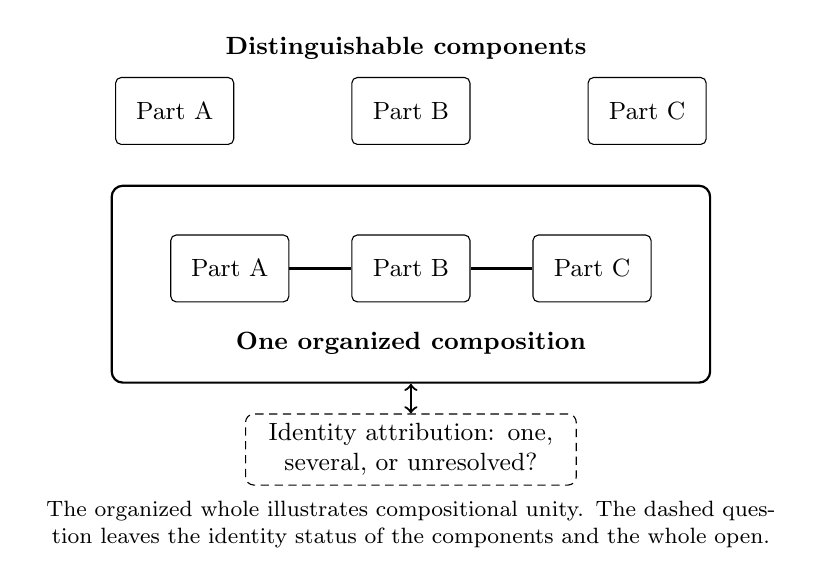
\begin{tikzpicture}[
    part/.style={
        draw,
        rounded corners=2pt,
        minimum width=1.5cm,
        minimum height=0.85cm,
        align=center,
        font=\small
    },
    whole/.style={
        draw,
        rounded corners=4pt,
        thick,
        minimum width=7.6cm,
        minimum height=2.5cm
    },
    question/.style={
        draw,
        densely dashed,
        rounded corners=3pt,
        minimum width=4.2cm,
        minimum height=0.9cm,
        align=center,
        text width=3.9cm,
        font=\small
    }
]

% Components considered separately
\node[part] (p1) at (-3.0,1.2) {Part A};
\node[part] (p2) at (0,1.2) {Part B};
\node[part] (p3) at (3.0,1.2) {Part C};

\node[align=center, font=\small\bfseries] at (0,2.0) {
    Distinguishable components
};

% Composed configuration
\node[whole] (frame) at (0,-1.0) {};

\node[part] (a) at (-2.3,-0.8) {Part A};
\node[part] (b) at (0,-0.8) {Part B};
\node[part] (c) at (2.3,-0.8) {Part C};

\draw[thick] (a) -- (b);
\draw[thick] (b) -- (c);

\node[font=\small\bfseries] at (0,-1.75) {
    One organized composition
};

% Identity question
\node[question] (identity) at (0,-3.1) {
    Identity attribution:
    one, several, or unresolved?
};

\draw[<->, thick] (frame.south) -- (identity.north);

\node[
    align=center,
    text width=9.5cm,
    font=\footnotesize
] at (0,-4.05) {
    The organized whole illustrates compositional unity.
    The dashed question leaves the identity status of
    the components and the whole open.
};

\end{tikzpicture}

\caption{Distinguishable components organized within one composition}
\label{fig:components-and-composed-configuration}

\end{figure}

% =============================================================================
% END OF ASSET IL01
% =============================================================================